\documentclass[border=3pt]{standalone}
% Preâmbulo compartilhado pelos diagramas TikZ da aula 11 (Localização por Grade e Monte Carlo)
\usepackage[T1]{fontenc}
\usepackage[utf8]{inputenc}
\usepackage{lmodern}
\usepackage{amsmath}
\usepackage{xcolor}
\usepackage{tikz}
\usetikzlibrary{arrows.meta,angles,quotes,decorations.pathmorphing,calc,
                positioning,shapes.geometric,shapes.misc,backgrounds,fit,
                math}

% Paleta (mesma dos SVGs originais)
\definecolor{dblue}{HTML}{2A5B8C}
\definecolor{dorange}{HTML}{B3541E}
\definecolor{dgreen}{HTML}{4A7C59}
\definecolor{dred}{HTML}{9C4B4B}
\definecolor{dcream}{HTML}{F4F1EA}
\definecolor{dshade}{HTML}{DDD7C9}

% Função gaussiana (não normalizada por padrão de escala visual)
\pgfmathdeclarefunction{gauss}{3}{%
  \pgfmathparse{1/(#3*sqrt(2*pi))*exp(-((#1-#2)^2)/(2*#3^2))}%
}

% Estilos comuns (prefixo d... para não colidir com chaves internas do pgf)
\tikzset{
  >={Stealth[length=2mm]},
  dguide/.style={gray!55, dashed, line width=0.4pt},
  daxis/.style={gray!60, line width=0.7pt, ->},
  dbody/.style={fill=black!3, draw=black!80, line width=1pt},
  dacc/.style={draw=dblue, line width=1pt},
  dlbl/.style={black!55, font=\small},
  dsub/.style={black!45, font=\footnotesize},
  dstate/.style={circle, draw=black!80, fill=dcream, line width=1pt,
                 minimum size=17mm, font=\large, inner sep=1pt},
  dobs/.style={circle, draw=black!80, fill=dshade, line width=1pt,
               minimum size=14mm, font=\large, inner sep=1pt},
  dbox/.style={rounded corners=2pt, draw=black!80, fill=dcream, line width=1pt,
               align=center, inner sep=6pt},
  dop/.style={circle, draw=black!80, fill=white, line width=1pt,
              minimum size=6mm, inner sep=0pt, font=\small},
  dtrans/.style={->, dblue, line width=1pt},
  dmeas/.style={->, dorange, line width=1pt},
  dcurve/.style={line width=1pt, dblue},
  dcurveb/.style={line width=1.4pt, dorange},
}

\begin{document}
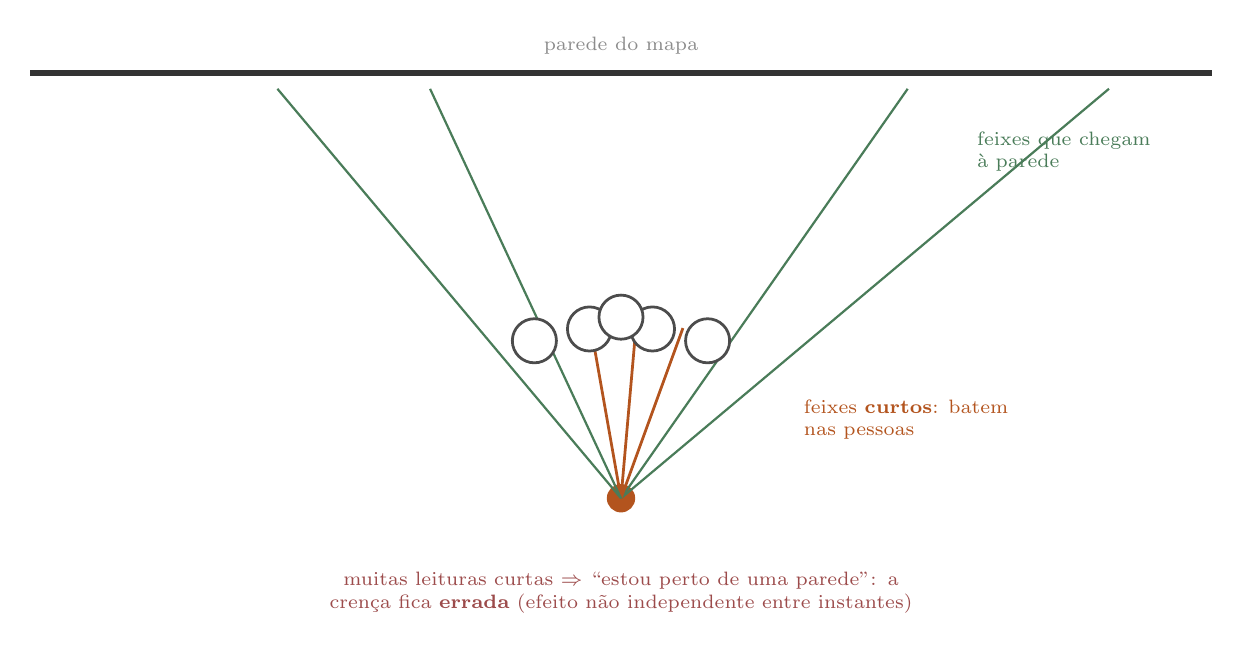
\begin{tikzpicture}[x=1cm,y=1cm]
  \draw[dbody, line width=2pt] (-2.5,5.4) -- (12.5,5.4);
  \node[dsub, font=\scriptsize] at (5,5.75) {parede do mapa};
  \fill[dorange] (5,0) circle (0.18);
  \foreach \a in {40,55,70,85,100,115,130} {
    \pgfmathsetmacro{\hit}{(\a>60 && \a<110)? 1 : 0}
    \ifnum\hit=1 \draw[dorange, line width=1pt] (5,0) -- ++(\a:2.3); \else \draw[dgreen, line width=0.8pt] (5,0) -- ++(\a:{5.2/sin(\a)}); \fi
  }
  \foreach \x/\y in {3.9/2.0,4.6/2.15,5.4/2.15,6.1/2.0,5.0/2.3} { \draw[black!70, fill=white, line width=1pt] (\x,\y) circle (0.28); }
  \node[dorange, font=\scriptsize, align=left, anchor=west] at (7.2,1.0) {feixes \textbf{curtos}: batem\\ nas pessoas};
  \node[dgreen, font=\scriptsize, align=left, anchor=west] at (9.4,4.4) {feixes que chegam\\ à parede};
  \node[dred, font=\scriptsize, align=center, text width=9.5cm] at (5,-1.2) {muitas leituras curtas $\Rightarrow$ ``estou perto de uma parede'': a crença fica \textbf{errada} (efeito não independente entre instantes)};
\end{tikzpicture}
\end{document}
